% ==================== 2.4.5 三重螺旋轴 ====================
\subsubsection{三重螺旋轴（\texorpdfstring{$P\,3_1$}{P3₁}）}

螺旋轴 $n_m$ 是旋转 $2\pi/n$ 与沿轴方向平移 $m/n$ 个晶格周期的联合操作，属于微观
对称元素。为观察 $3_1$ 螺旋轴（旋转 $120^\circ$ 并沿轴平移 $1/3$ 个周期），选用空间群
$P\,3_1$（No.~144，三方晶系），建模参数见表~\ref{tab:sym-screw31}。

\begin{table}[H]
  \centering
  \caption{三重螺旋轴演示的建模参数}
  \label{tab:sym-screw31}
  \begin{tabular}{ll}
    \toprule
    项目 & 参数 \\
    \midrule
    空间群 & $P\,3_1$（No.~144，三方晶系） \\
    晶格常数 & $a=b=c=5.0$\,\AA，$\alpha=\beta=90^\circ$，$\gamma=120^\circ$ \\
    原子坐标 & Si：$(0.2,\,0.3,\,0.4)$（一般位置） \\
    等效位置数 & 3（单胞内 3 个原子，高度各不相同） \\
    \bottomrule
  \end{tabular}
\end{table}

\begin{figure}[H]
  \centering
  \subcaptionbox{空间群与晶胞参数设置}{%
    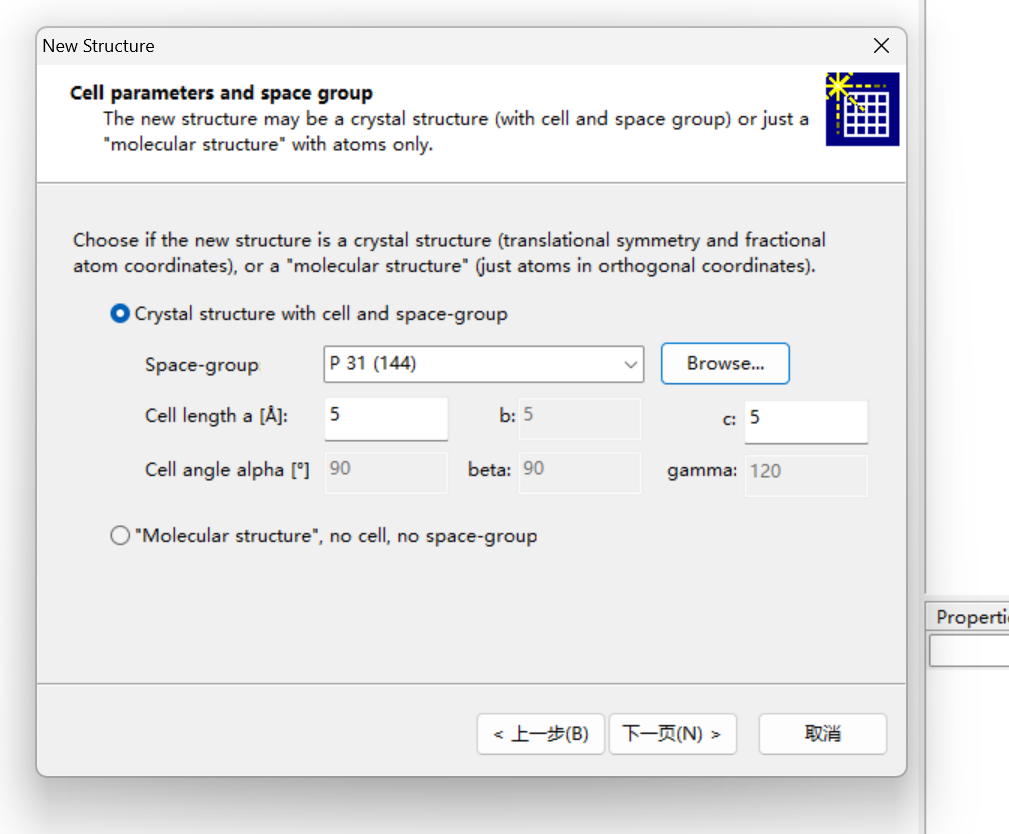
\includegraphics[width=0.44\textwidth]{assets/symmetry/screw31/a.png}}
  \hfill
  \subcaptionbox{非对称单元原子（Si）添加}{%
    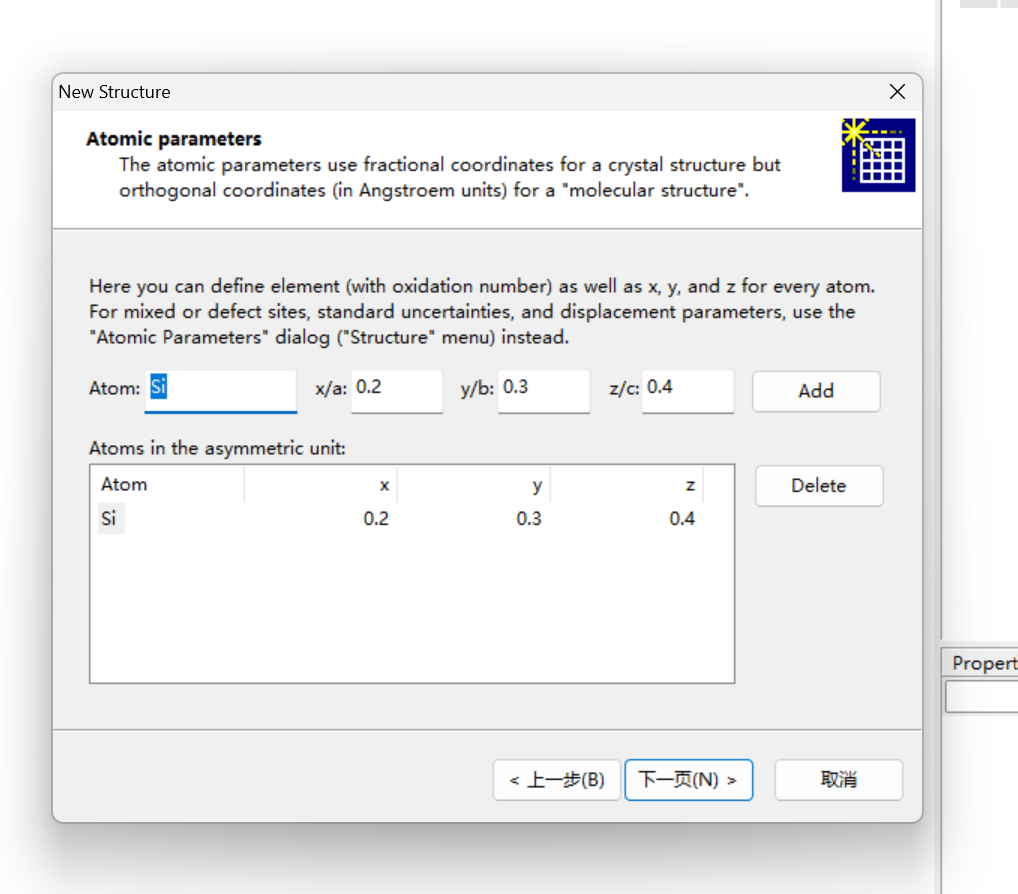
\includegraphics[width=0.44\textwidth]{assets/symmetry/screw31/b.png}}
  \caption{三重螺旋轴（$P\,3_1$）演示的参数设置}
  \label{fig:sym-screw31-param}
\end{figure}

\begin{figure}[H]
  \centering
  \subcaptionbox{单胞图：3 个原子高度各不相同、呈螺旋排列}{%
    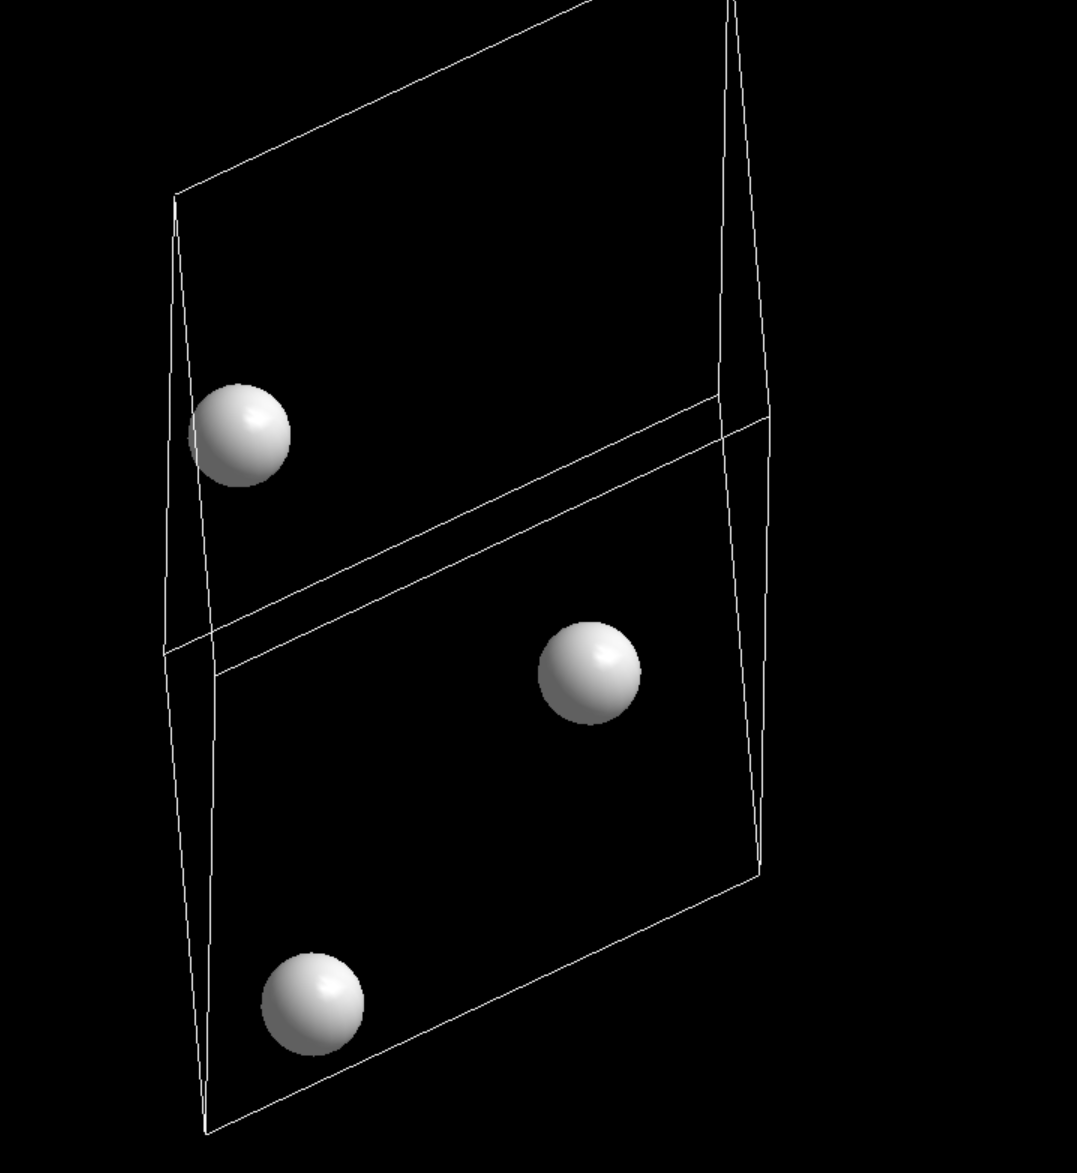
\includegraphics[width=0.44\textwidth]{assets/symmetry/screw31/c.png}}
  \hfill
  \subcaptionbox{超晶胞图：沿 $c$ 轴方向延伸的螺旋链}{%
    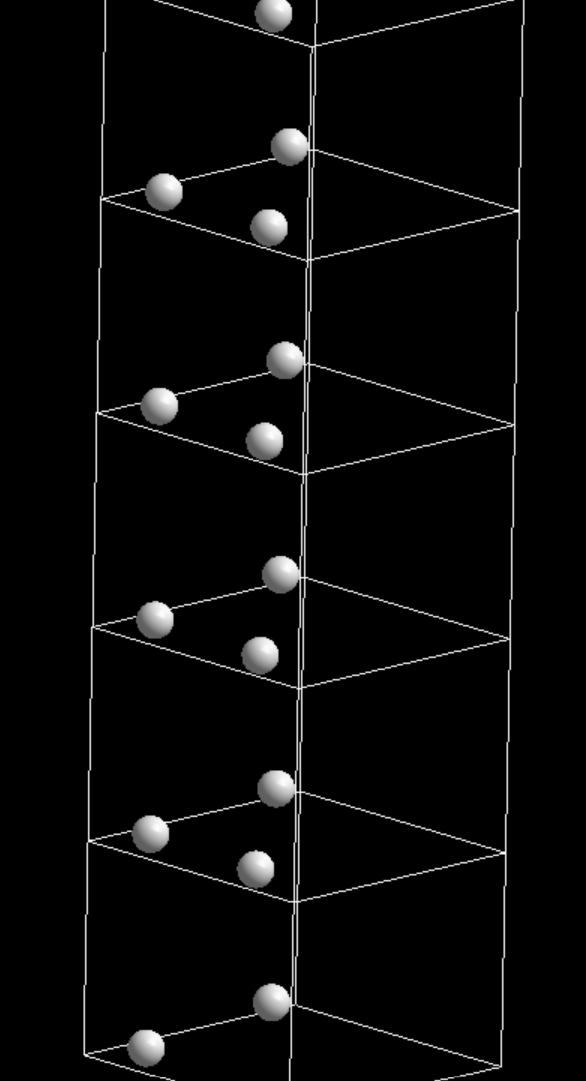
\includegraphics[width=0.44\textwidth]{assets/symmetry/screw31/d.png}}
  \caption{三重螺旋轴（$P\,3_1$）的单胞与超晶胞模型}
  \label{fig:sym-screw31-model}
\end{figure}

$P\,3_1$ 的一般位置等效位置为 $(x,y,z)$、$(\bar y,\,x-y,\,z+\tfrac13)$ 与
$(-x+y,\,\bar x,\,z+\tfrac23)$：操作一次得到 1 个原子，共操作 3 次、生成 3 个原子。
将 Si 的坐标 $(0.2,0.3,0.4)$ 代入，3 个原子的分数坐标为 $(0.2,0.3,0.4)$、
$(0.7,0.9,0.733)$ 与 $(0.1,0.8,0.067)$：三者高度（$z$ 坐标）依次相差 $1/3$，沿 $c$
轴呈螺旋上升排列，不位于同一平面（图~\ref{fig:sym-screw31-model}(a)）；执行第 3 次
操作时，原子回到与初始位置等效的位置 $(0.2,0.3,1.4)$——即绕轴旋转一周的同时沿 $c$
方向平移了 1 个晶胞周期，因此在超晶胞中沿 $c$ 轴可以看到连续的螺旋链
（图~\ref{fig:sym-screw31-model}(b)）。

\textbf{特征与辨识要点。}螺旋轴与纯旋转轴的本质区别在于是否含沿轴方向的平移分量：
3 次旋转轴的 3 个原子位于同一平面（2.4.2 节），而 $3_1$ 螺旋轴的 3 个原子依次升高
$c/3$、呈螺旋排列。螺旋轴 $n_m$ 的 $m$ 不同，平移分量为 $m/n$ 个周期；$3_1$ 与
$3_2$ 的平移方向与旋转方向组合相反，互为对映关系（右旋与左旋）。螺旋轴属微观对称
元素，只能存在于无限晶体中，实际晶体中十分常见，例如 $\alpha$-石英的 $P\,3_1\,2\,1$
与 $P\,3_2\,2\,1$ 就互为含 $3_1$、$3_2$ 螺旋轴的一对对映空间群。
